\documentclass[tikz,border=3pt]{standalone}
\usepackage{amsmath,amssymb}
\usepackage{lmodern}
\usetikzlibrary{arrows.meta,shapes.geometric,calc}
% Generated from the manuscript AUX; rerun after equation moves.
\newcommand{\EqSearch}{13} % eq:lscbo_search
\newcommand{\EqRotation}{14} % eq:lscbo_rotation
\newcommand{\EqAttack}{15} % eq:lscbo_attack
\newcommand{\EqLevy}{18} % eq:lscbo_levy
\newcommand{\EqAccept}{19} % eq:pareto_accept
\newcommand{\EqExec}{1} % eq:exec_time
\newcommand{\EqReference}{6} % eq:reference
\newcommand{\EqObjective}{7} % eq:objective
\newcommand{\EqEnergy}{2} % eq:energy
\newcommand{\EqImbalance}{5} % eq:lbr
\newcommand{\EqDecoder}{20} % eq:decoder
\newcommand{\FigMechanism}{1} % fig:mechanism_workflow
\newcommand{\AlgCloud}{2} % alg:lscbo

\definecolor{ink}{HTML}{34495E}
\definecolor{bluefill}{HTML}{EBF3FA}
\definecolor{greenfill}{HTML}{EAF4EC}
\definecolor{purplefill}{HTML}{F2EDF8}
\definecolor{fitnessfill}{HTML}{FFF3DA}
\tikzset{
flow/.style={-{Latex[length=1.8mm]},draw=ink,line width=.5pt},
dataflow/.style={-{Latex[length=1.8mm]},draw=green!35!black,dashed,line width=.6pt},
box/.style={draw=ink,rounded corners=1pt,fill=bluefill,align=center,
font=\sffamily\fontsize{9}{11}\selectfont,text width=46mm,inner sep=1.5mm},
decision/.style={diamond,aspect=3.8,draw=ink,fill=white,align=center,
font=\sffamily\fontsize{8.5}{10}\selectfont,text width=29mm,inner sep=.3mm},
tag/.style={font=\sffamily\fontsize{8.5}{10}\selectfont,fill=white,inner sep=.4mm}
}
\begin{document}
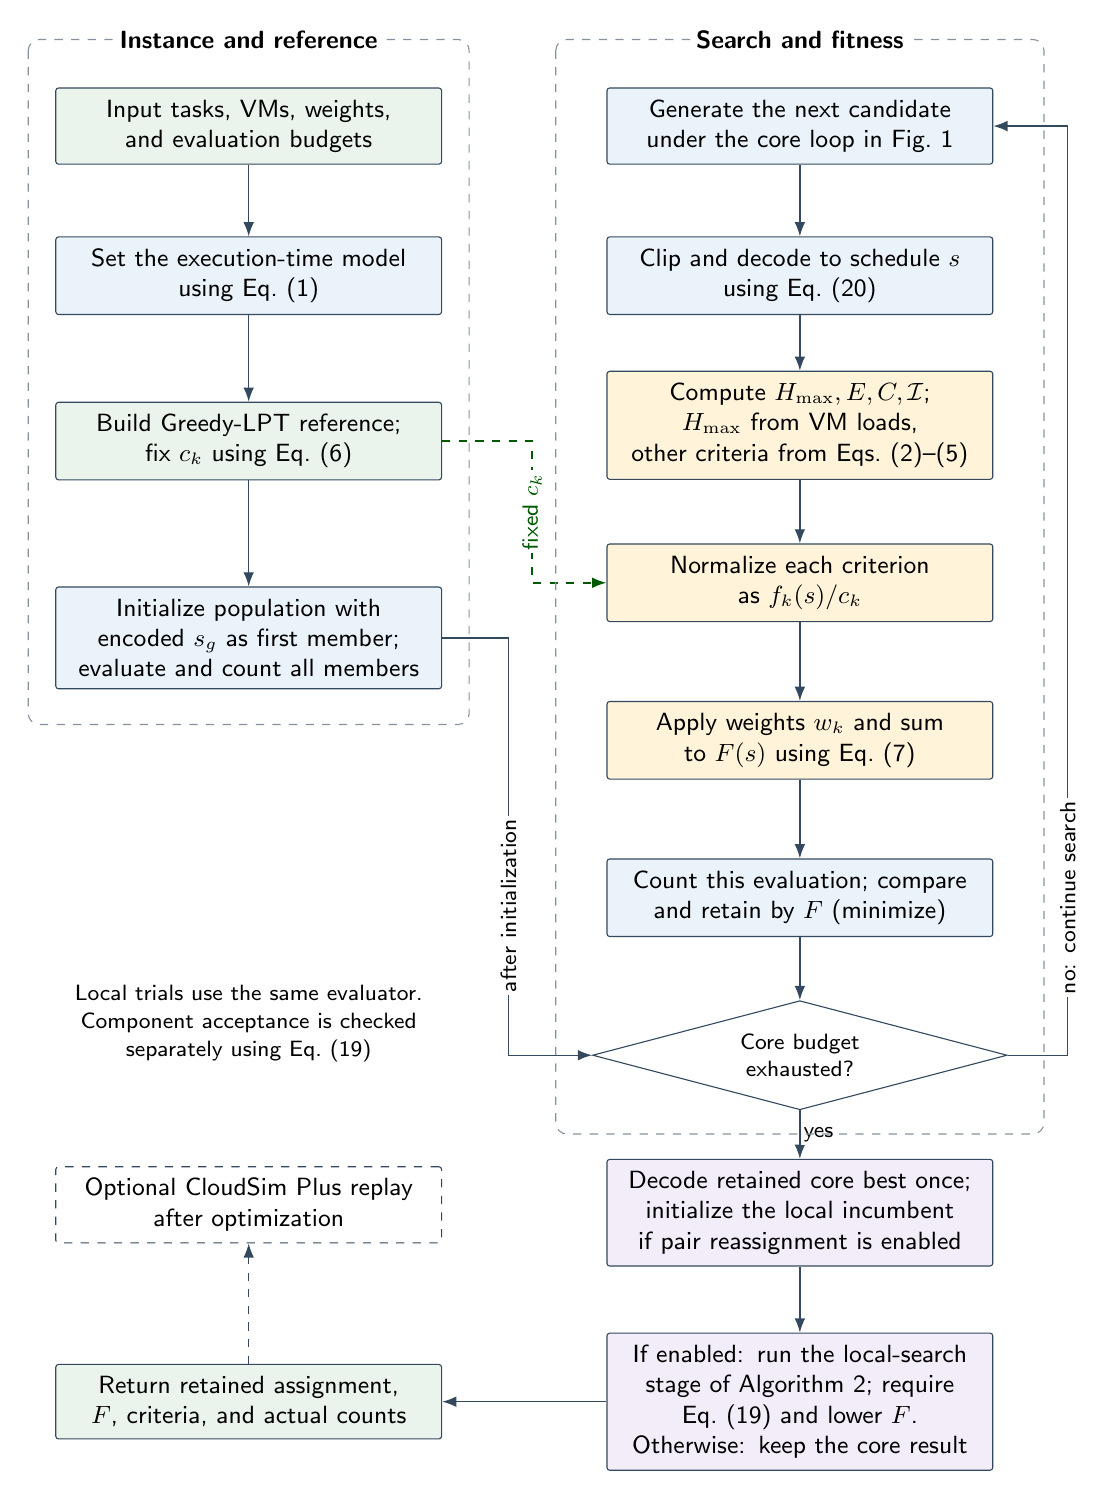
\begin{tikzpicture}[x=1mm,y=-1mm]
\node[box,fill=greenfill] (input) at (29,0) {Input tasks, VMs, weights,\\and evaluation budgets};
\node[box] (instance) at (29,19) {Set the execution-time model\\using Eq.~(\EqExec)};
\node[box,fill=greenfill] (reference) at (29,40) {Build Greedy-LPT reference;\\fix $c_k$ using Eq.~(\EqReference)};
\node[box] (encode) at (29,65) {Initialize population with\\encoded $s_g$ as first member;\\evaluate and count all members};
\node[box] (core) at (99,0) {Generate the next candidate\\under the core loop in Fig.~\FigMechanism};
\node[box] (decode) at (99,19) {Clip and decode to schedule $s$\\using Eq.~(\EqDecoder)};
\node[box,fill=fitnessfill] (metrics) at (99,38) {Compute $H_{\mathrm{max}},E,C,\mathcal{I}$;\\$H_{\mathrm{max}}$ from VM loads,\\other criteria from Eqs.~(\EqEnergy)--(\EqImbalance)};
\node[box,fill=fitnessfill] (normalize) at (99,58) {Normalize each criterion\\as $f_k(s)/c_k$};
\node[box,fill=fitnessfill] (score) at (99,78) {Apply weights $w_k$ and sum\\to $F(s)$ using Eq.~(\EqObjective)};
\node[box] (retain) at (99,98) {Count this evaluation; compare\\and retain by $F$ (minimize)};
\node[decision] (budget) at (99,118) {Core budget\\exhausted?};
\node[box,fill=purplefill] (handoff) at (99,138) {Decode retained core best once;\\initialize the local incumbent\\if pair reassignment is enabled};
\node[box,fill=purplefill] (local) at (99,162) {If enabled: run the local-search\\stage of Algorithm~\AlgCloud; require\\Eq.~(\EqAccept) and lower $F$.\\Otherwise: keep the core result};
\node[box,fill=greenfill] (output) at (29,162) {Return retained assignment,\\$F$, criteria, and actual counts};
\node[box,fill=white,dashed] (replay) at (29,137) {Optional CloudSim Plus replay\\after optimization};
\node[tag,align=center] at (29,114) {Local trials use the same evaluator.\\Component acceptance is checked\\separately using Eq.~(\EqAccept)};
\draw[flow] (input) -- (instance);
\draw[flow] (instance) -- (reference);
\draw[flow] (reference) -- (encode);
\draw[flow] (encode.east) -- (62,65) -- (62,118) -- (budget.west);
\node[tag,rotate=90] at (62,99) {after initialization};
\draw[dataflow] (reference.east) -- (65,40) -- (65,58) -- (normalize.west);
\node[tag,rotate=90,text=green!35!black] at (65,49) {fixed $c_k$};
\draw[flow] (core) -- (decode);
\draw[flow] (decode) -- (metrics);
\draw[flow] (metrics) -- (normalize);
\draw[flow] (normalize) -- (score);
\draw[flow] (score) -- (retain);
\draw[flow] (retain) -- (budget);
\draw[flow] (budget.east) -- (133,118) -- (133,0) -- (core.east);
\node[tag,rotate=90] at (133,98) {no: continue search};
\draw[flow] (budget) -- node[tag,right]{yes} (handoff);
\draw[flow] (handoff) -- (local);
\draw[flow] (local) -- (output);
\draw[flow,dashed] (output) -- (replay);
\draw[dashed,rounded corners,draw=ink!60] (1,-11) rectangle (57,76);
\draw[dashed,rounded corners,draw=ink!60] (68,-11) rectangle (130,128);
\node[tag,font=\sffamily\bfseries\small] at (29,-11) {Instance and reference};
\node[tag,font=\sffamily\bfseries\small] at (99,-11) {Search and fitness};
\end{tikzpicture}
\end{document}
